\documentclass[10pt, a4paper]{article}

\usepackage[english]{babel}
\usepackage[utf8]{inputenc}
\usepackage{float}
\usepackage[]{amsmath} 
\usepackage{graphicx}

% Define question and answer command
\newcounter{qcounter}
\newcommand{\q}[2]
{
    \textbf{Task \refstepcounter{qcounter} \arabic{qcounter}: #1} \\
    #2
    \par
    \vspace{0.5cm}
} 

\begin{document}

\begin{titlepage}
\centering
{
 \scshape \LARGE 
EL2450 Homework 2
}
\vfill
Andreas Fr\"{o}derberg - 19880730-7577
\par
Martin Favre - 19920130-0010
\end{titlepage}

\section{Rate Monotonic scheduling}
\label{sec:rate_monotonic_scheduling}

\q %1
{
    Explain what Rate Monotonic scheduling means.
}
{
    In Rate Monotonic scheduling, each task is given a fixed priority based on
    its task rate, shorter task rate equals higher priority. The task with the
    highest priority is then run at all times.
}

\q %2
{
	Are the three tasks schedulable?
}
{
	Calculating the utilization factor U from 
	\begin{equation}
		U = \sum\limits_{i=1}^n \frac{C_i}{T_i}=\frac{6}{20} + \frac{6}{29} +
        \frac{6}{35} = 0.68
	\end{equation}	
    To be schedulable, the condition 
    \begin{equation}
        U \leq n(2^{\frac{1}{n}} - 1),
    \end{equation}
    where $n$ is the number of processes. Calculating for this example with 3
    tasks, the condition becomes
    \begin{equation}
        \label{eq:ut_rm}
        0.68 \leq 3(2^{\frac{1}{3}} - 1)=0.78
    \end{equation}
    which holds, therefore the taskset is schedulable with RM scheduling.
}
\q %3
{
    What are the differences in control performance between the different
    pendulums?
}
{
    All pendulums are asymptotically stable and have similar control
    performance. The performance is shown in Figure~\ref{fig:T3_dmperformance}.
    \begin{figure}[H]
        \centering
        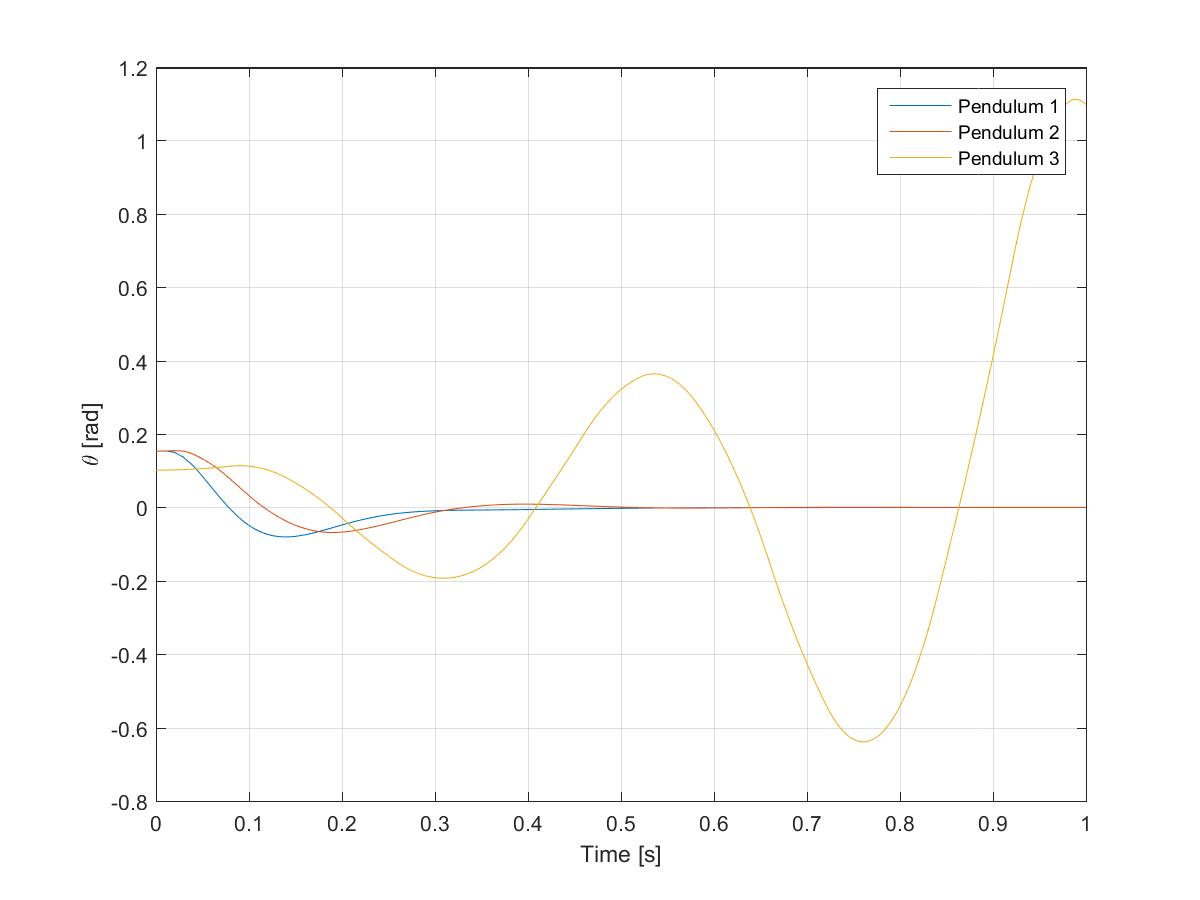
\includegraphics[width=1\linewidth]{../Matlab/HW2_sources_Windows64bit/images/Task_3_dm_performance.png}
        \caption{Performance of pendulums under rate monotonic scheduling.}
        \label{fig:T3_dmperformance}
    \end{figure}
}
\q %4
{
    Compare against the schedule in the model. Does it match?
}
{
    In Figure~\ref{fig:Task_4_sch_6ms}, the execution of tasks in Matlab is
    shown.
    \begin{figure}[H]
        \centering
        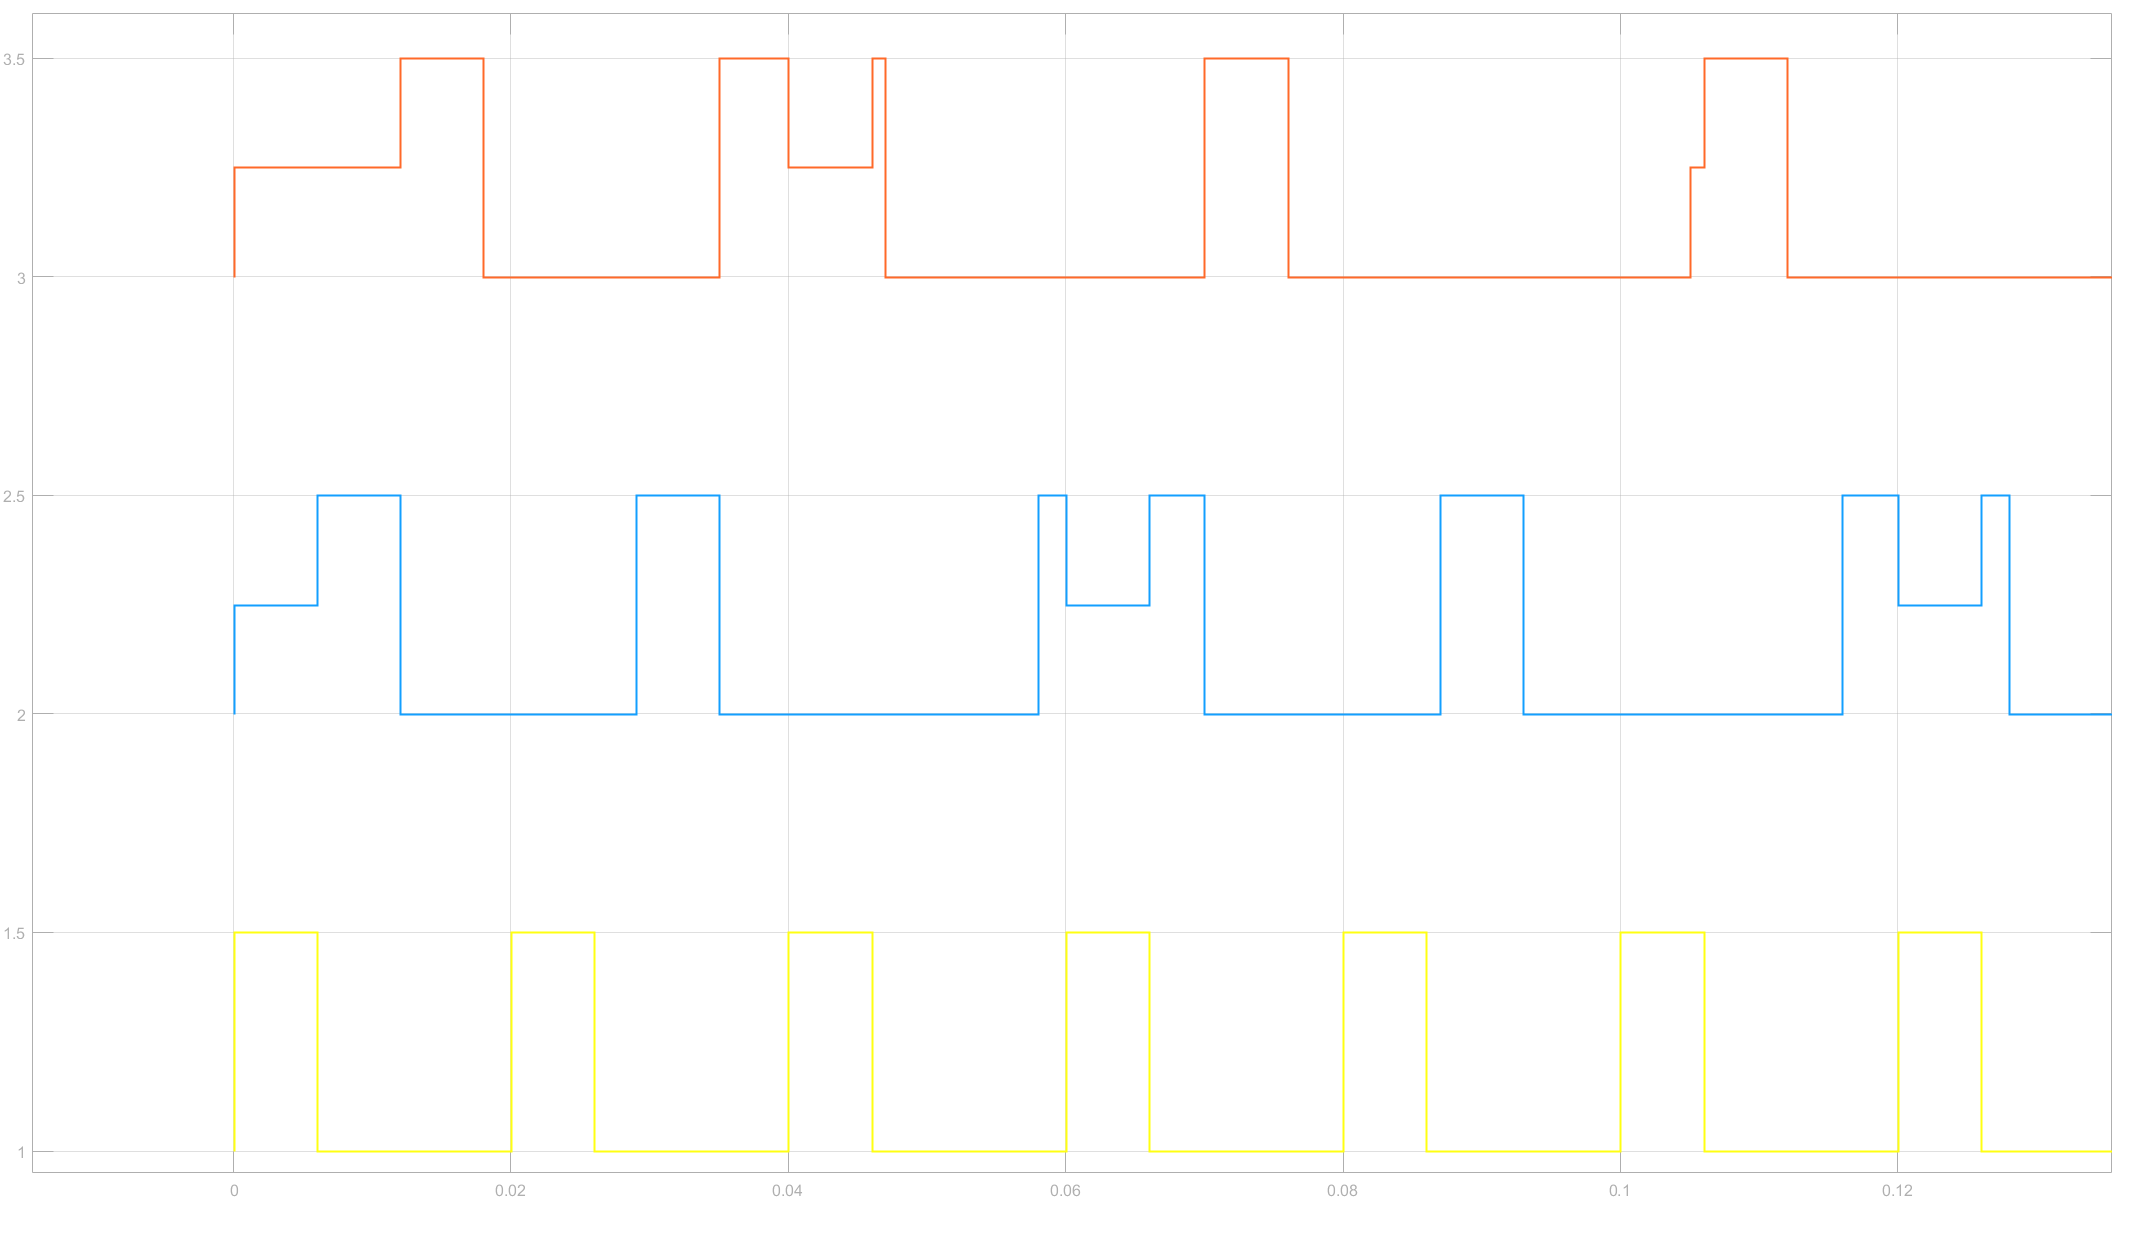
\includegraphics[width=1\linewidth]{../Matlab/HW2_sources_Windows64bit/images/Task_4_sch_6ms.png}
        \caption{Schedule for pendulums when computation time of all is 6 ms.
        Yellow is small pendulum, blue is medium and red is big.}
        \label{fig:Task_4_sch_6ms}
    \end{figure}
    In the figure below, Figure~\ref{fig:Task_4_sch_6ms_drawn}, the execution
    order as calculated by hand is shown.
    \begin{figure}[htpb]
        \centering
        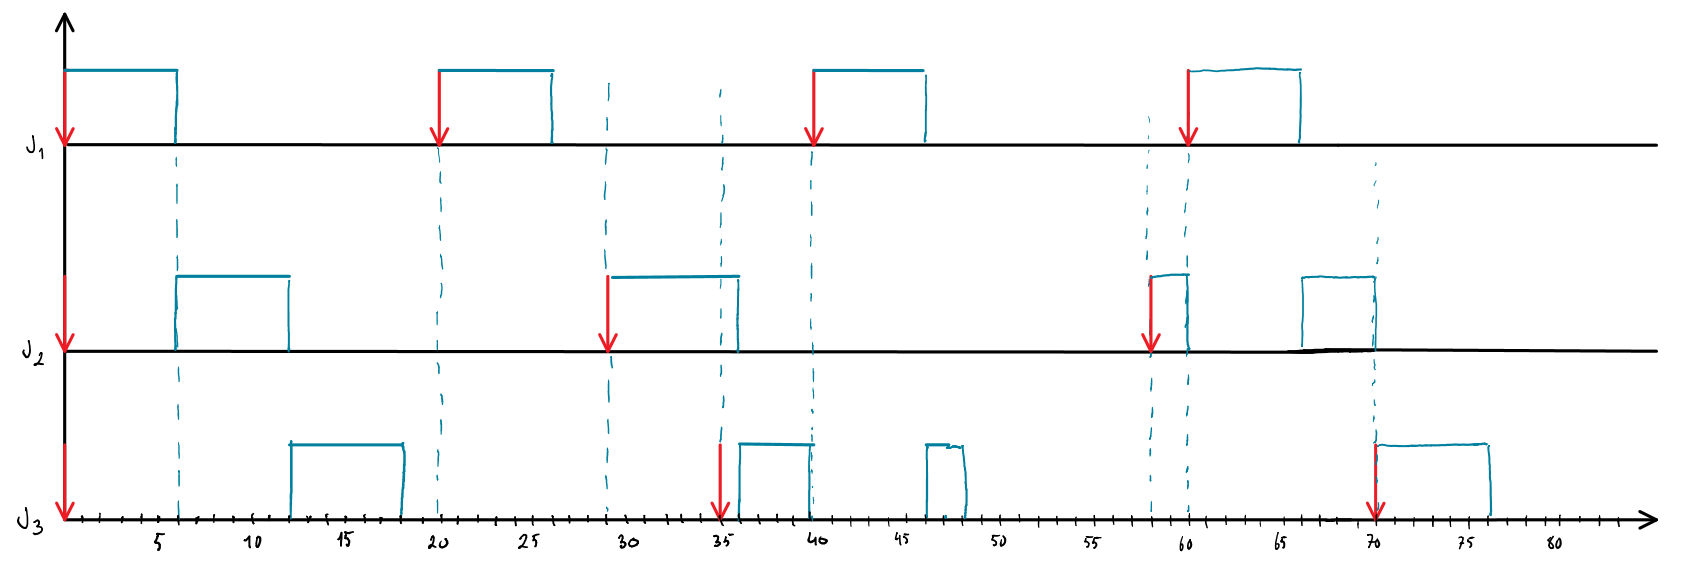
\includegraphics[width=1\linewidth]{../Matlab/HW2_sources_Windows64bit/images/rm_tasks.PNG}
        \caption{Hand drawn and calculated execution order with Rate Monotonic
        scheduling. Task $J_1$ represents the small pendulum and rising index
        represents bigger pendulums.}
        \label{fig:Task_4_sch_6ms_drawn}
    \end{figure}
    It can be seen that the schedules both are consistent.
}
    
\q %5
{
    Setting the execution time for all three processes to 10ms, what are the
differences with respect to control performance?
}
{
    For this execution time, the CPU utilization factor becomes
    \begin{equation}
		U = \sum\limits_{i=1}^n \frac{C_i}{T_i}=\frac{10}{20} + \frac{10}{29} +
        \frac{10}{35} = 1.1.
    \end{equation}
    The utilization factor is thus larger than Equation~\ref{eq:ut_rm} which
    means that the processes is not schedulable. This is seen in
    Figure~\ref{fig:Task_5_dm_performance} where the small pendulum is no
    longer stable because of the fact that the deadlines are missed.
	\begin{figure}[H]
        \centering
        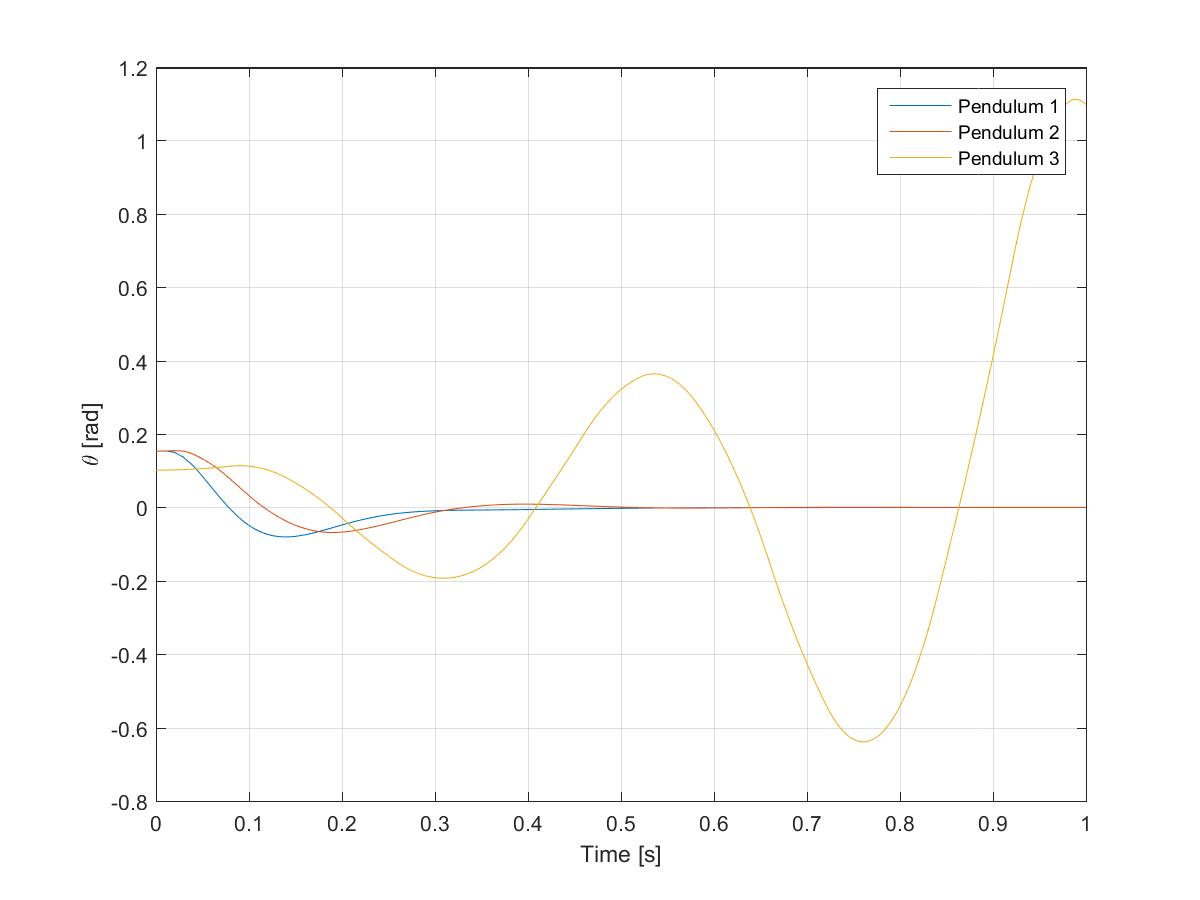
\includegraphics[width=1\linewidth]{../Matlab/HW2_sources_Windows64bit/images/Task_5_dm_performance.png}
        \caption{Performance of pendulums under rate monotonic schedulingi
        with computation time 10 ms for each task.}
        \label{fig:Task_5_dm_performance}
    \end{figure}
    The schedule in the simulations is shown in
    Figure~\ref{fig:Task_5_sch_10ms}.
    \begin{figure}[H]
        \centering
        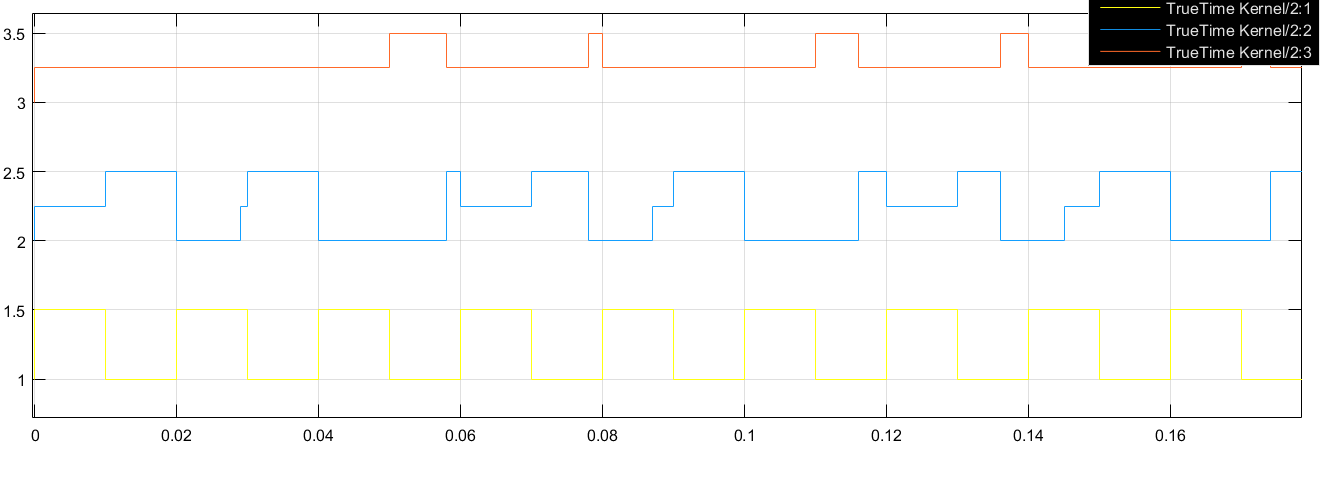
\includegraphics[width=1\linewidth]{../Matlab/HW2_sources_Windows64bit/images/Task_5_sch_10ms.png}
        \caption{Schedule for Rate Monotonic scheduling when computation time is
        10 ms}
        \label{fig:Task_5_sch_10ms}
    \end{figure}
    When viewing the hand-drawn and the real schedule, the following are shown.
    \begin{figure}[H]
        \centering
        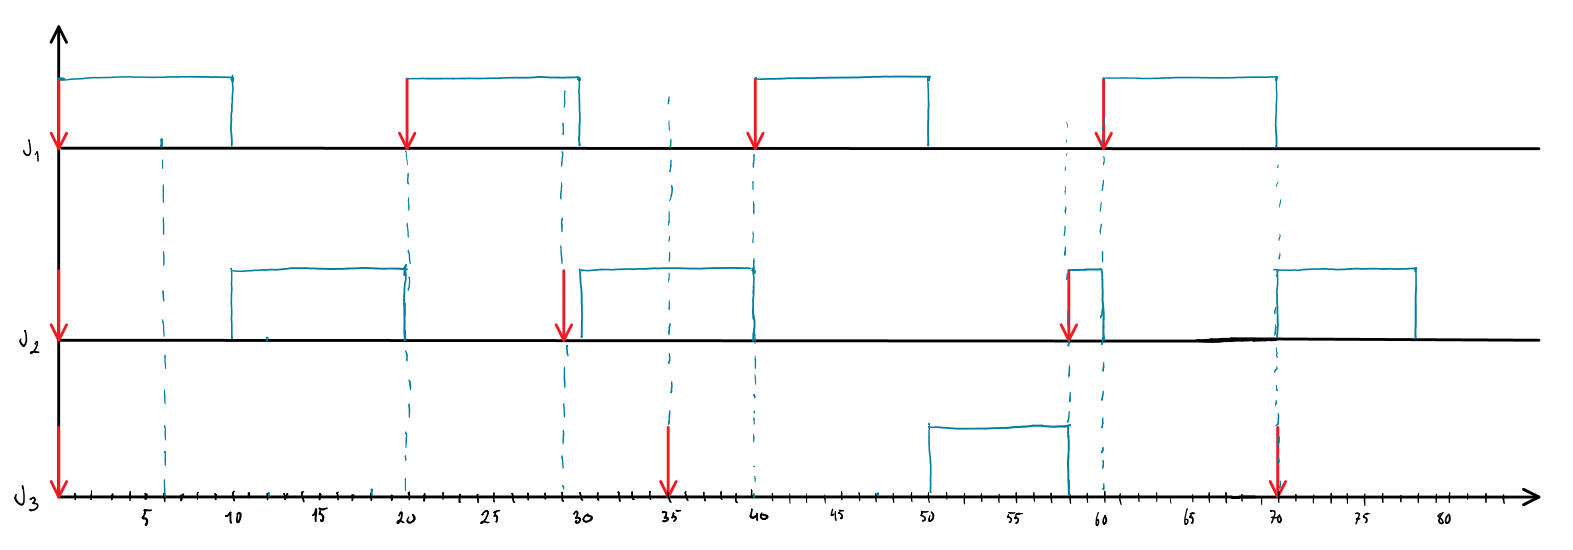
\includegraphics[width=1\linewidth]{../Matlab/HW2_sources_Windows64bit/images/rm_tasks_10ms.PNG}
        \caption{Schedule when computation time is 10 ms. Task $J_1$ is smallest
        pendulum, higher index represents larger pendulum.}
        \label{fig:Task_5_rm_performance_hand}
    \end{figure}

}
%% Earliest deadline first
\section{Earliest Deadline First, EDF}
\label{sec:earliest_deadline_first_edf}
% Reset the task counter
\setcounter{qcounter}{0}
\q %1
{
    Explain how EDF works. What are the advantages and disadvantages of the
    approach compared to RM?
}
{
    In EDF, the task that has the closest deadline to the current time is always
    run. The advantage of this is that the processor can be fully utilized if
    the the scheme is schedulable. Another advantage is that tasks will not get
    starved if the processor is overloaded and deadlines are missed since the
    dynamic prioritization will handle allow all tasks to get processing time.
    One disadvantage is that tasks can not be given predefined priorities which
    might be important depending on the implementation.
}
\q %2
{
    Assume the execition time is changed back to 6 ms. Are the tasks schedulable
    with the EDF? Please motivate your answer and costruct part of the
    corresponding schedule manually.
}
{
   	EDF is schedulable as long as CPU utilization is lower than 100 \%. The
    utilization factor is the same as the answer q2 from RM, 0.68. Since
    $U=0.68 \leq 1$ holds, the task set is schedulable with EDF.
    The hand calculated schedule is shown below in
    Figure~\ref{fig:6ms_sch_edf_hand}.
    \begin{figure}[H]
        \centering
        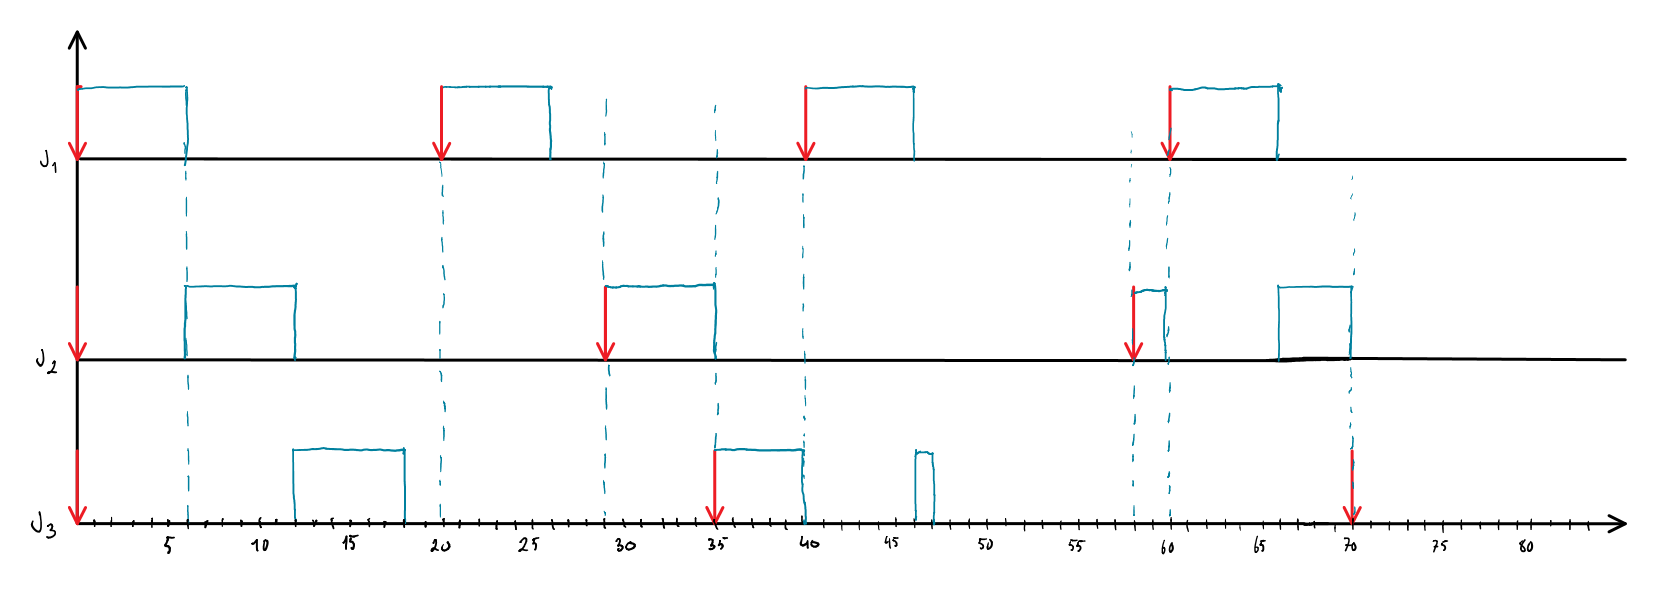
\includegraphics[width=1\linewidth]{../Matlab/HW2_sources_Windows64bit/images/Task_4_sch_6ms_edf.png}
        \caption{Schdule for EDF with 6 ms calculation time. Task $J_1$
        represents the smallest pendulum, higher index represents larger
        pendulums.}
        \label{fig:6ms_sch_edf_hand}
    \end{figure}
}

\q %3
{
    Using EDF - what are the differences in control performance between the
    different pendulums?
}
{
 		All pendulums are asymptotically stable and have similar control
    	performance. The performance is shown in Figure~\ref{fig:T3_dmperformance}.
		\begin{figure}[H]
    		\centering
        	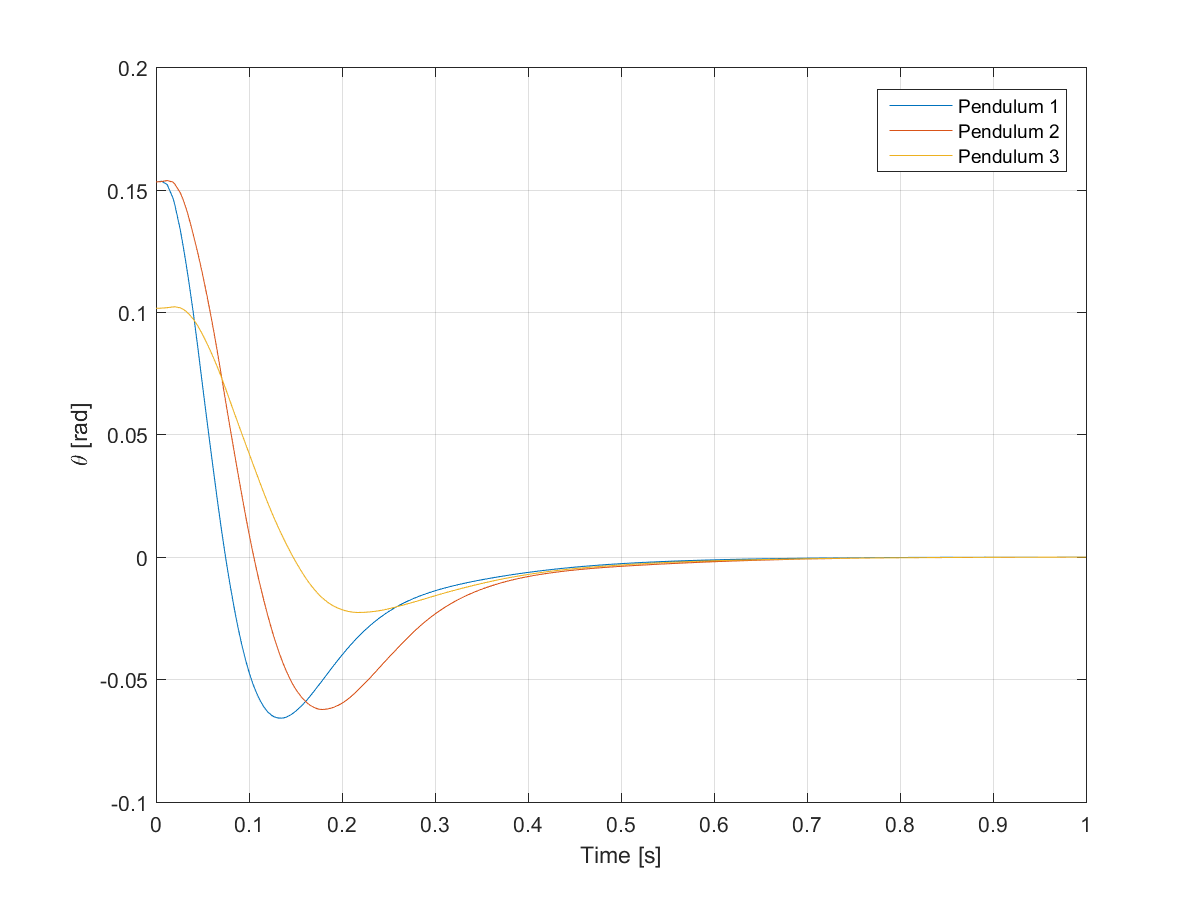
\includegraphics[width=1\linewidth]{../Matlab/HW2_sources_Windows64bit/images/Task_3_edf_performance.png}
            \caption{Performance of pendulums under earliest deadline first
            scheduling with computation time 6 ms for each task.}
        	\label{fig:Task_3_edf_performance}
    	\end{figure}
}

\q % 4
{
	Compare against the schedule in the model. Does it match?
}
{
	The schedule in the model is shown in Figure~\ref{fig:6ms_sch_edf}.
    \begin{figure}[H]
        \centering
        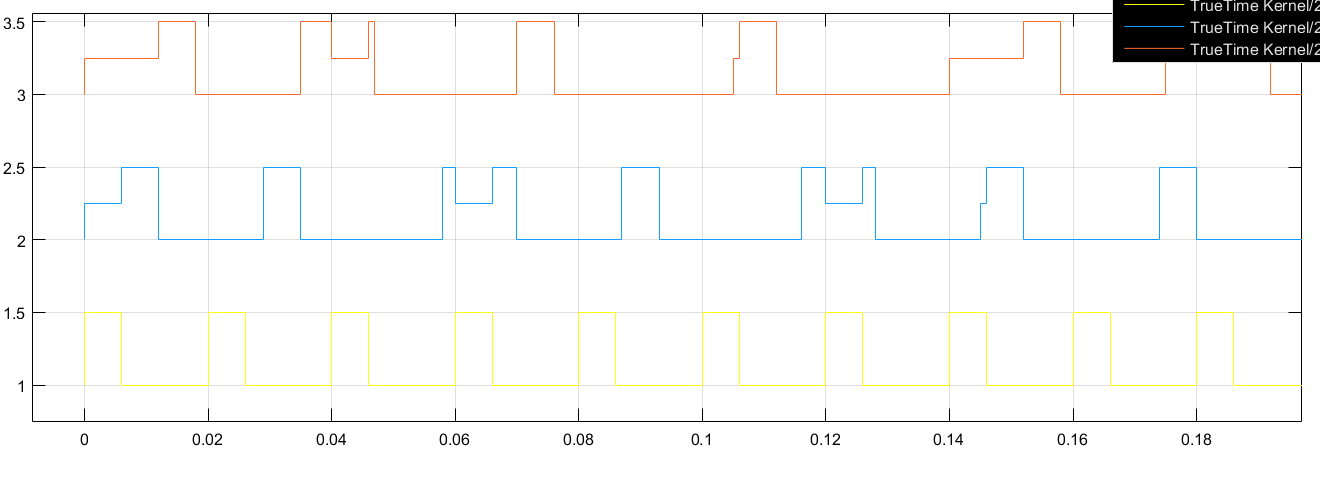
\includegraphics[width=1\linewidth]{../Matlab/HW2_sources_Windows64bit/images/Task_3_sch_6ms_edf.png}
        \caption{Performance of pendulums under earliest deadline first
        scheduling with computation time 6 ms for each task.}
        \label{fig:6ms_sch_edf}
    \end{figure}
    It is consistent with the schedule presented in task 2.
}
\q %5
{
	 Setting the execution time for all three processes to 10ms, what are the
differences with respect to control performance?
}
{
	For this execution time, the CPU utilization factor becomes
    \begin{equation}
		U = \sum\limits_{i=1}^n \frac{C_i}{T_i}=\frac{10}{20} + \frac{10}{29} +
        \frac{10}{35} = 1.1.
    \end{equation}
    The utilization factor is thus larger than one which means that the
    processes is not schedulable. 
	
	However looking at Figure~\ref{fig:Task_5_edf_performance} the system is still stable although with deteriorated 
	control performace for all three pendulums. This is a result of the disability to meet all the deadlines but still meeting enough for the system to stabilize. 


	\begin{figure}[H]
    		\centering
        	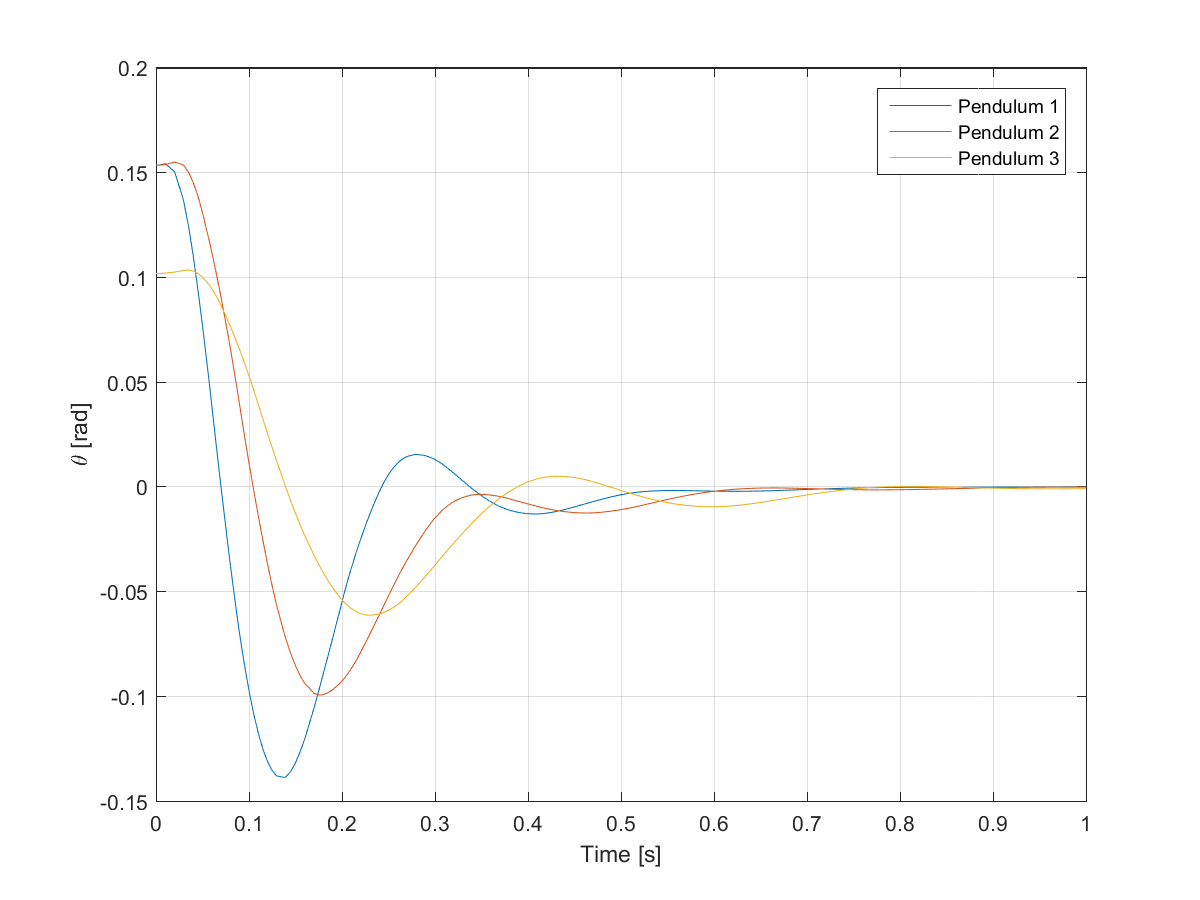
\includegraphics[width=1\linewidth]{../Matlab/HW2_sources_Windows64bit/images/Task_5_edf_performance.png}
        	\caption{Performance of pendulums under earliest deadline first scheduling
           	 with computation time 10 ms for each task.}
        	\label{fig:Task_5_edf_performance}
    	\end{figure}
}

\q % 6
{
	Does the controllers perform better with EDF compared to RM-scheduling?
}
{
	Comparing the systems with 6 $ms$ execution time in Figure~\ref{fig:T3_dmperformance} and Figure~\ref{fig:Task_3_edf_performance} little difference can
 	be seen. However with execution time of 10 $ms$ in Figure~\ref{fig:Task_5_dm_performance} and Figure~\ref{fig:Task_5_edf_performance} the control 
	performance is much better with EDF-scheduling.
	
	%Osäker på det här svaret - Vill dra en relation med U
	A relation can be drawn with the different utilization factors of EDF and RM, where RM is limited to a factor of 0.68 from Q2 whilst EDF can handle 1.0 and is 		 	therefore better. 
}

%% NETWORKED CONTROL SYSTEMS %% SKYNET HERE WE GO %%
\section{Networked Control Systems}
\label{sec:networked_control_systems}
% Reset the task counter
\setcounter{qcounter}{0}
\q % 1
{
	Do analytical calculations of the closed-loop equations.
}
{ %% Haveriet
	With
	\begin{equation}
		\dot{x}(t) = Iu(t) 
	\end{equation}
	\begin{equation}
		y(t) = Cx(t) 
	\end{equation}
	and
	\begin{equation}
		u(kh) = -Kx(kh).
	\end{equation}
	Sampling the system with a period h gives:
	\begin{equation}
		\Phi = e^{Ah}
	\end{equation}
	\begin{equation}
		\Gamma_0(\tau_A) = I\int_0^{h-\tau_k} \! \, \mathrm{d}s = (h-\tau_k)I
	\end{equation}
	\begin{equation}
		\Gamma_1(\tau_A) = I\int_{h-\tau_k}^{h} \! \, \mathrm{d}s = -\tau_kI
	\end{equation}
	Defining $z(kh) = [x^T(kh), u^T((k-1)h]^T$ as the augumented state vector, the augmented closed-loop system is
	\begin{equation}
		z((k+1)h) = \widetilde{\phi}(k)z(kh)
	\end{equation}	
	where
	\begin{equation}
		\widetilde{\phi}(k) = 
		\begin{bmatrix}
			\Phi-\Gamma_0(\tau_k)K & \Gamma_1(\tau_k) \\
			-K & 0
		\end{bmatrix}
		=
	\begin{bmatrix}
		1-(h-\tau_A)I & -\tau_AI \\
		-K & 0
	\end{bmatrix}
	.
	\end{equation}
	Which results in:
	\begin{equation}
		z((k+1)h) = 
	\begin{bmatrix}
		1-(h-\tau_A)I & -\tau_AI \\
		-K & 0
	\end{bmatrix}
		z(kh).
	\end{equation}

}
\q % 2
{
	Calculate stuff
}
{
	Present stuff
}

%% DISCRETE EVENT SYSTEMS %% SEXUAL DELAYS %%
\section{Discrete Event Systems}
\label{sec:discrete_event_systems}
% Reset the task counter
\setcounter{qcounter}{0}
\q % 1
{
	Construct and draw the DES that models $M_1$, $M_2$ and the $Buffer$
}
{

	In Figure~\ref{fig:task41_Chart}  the three systems can be seen.
	\begin{figure}[H]
    		\centering
        	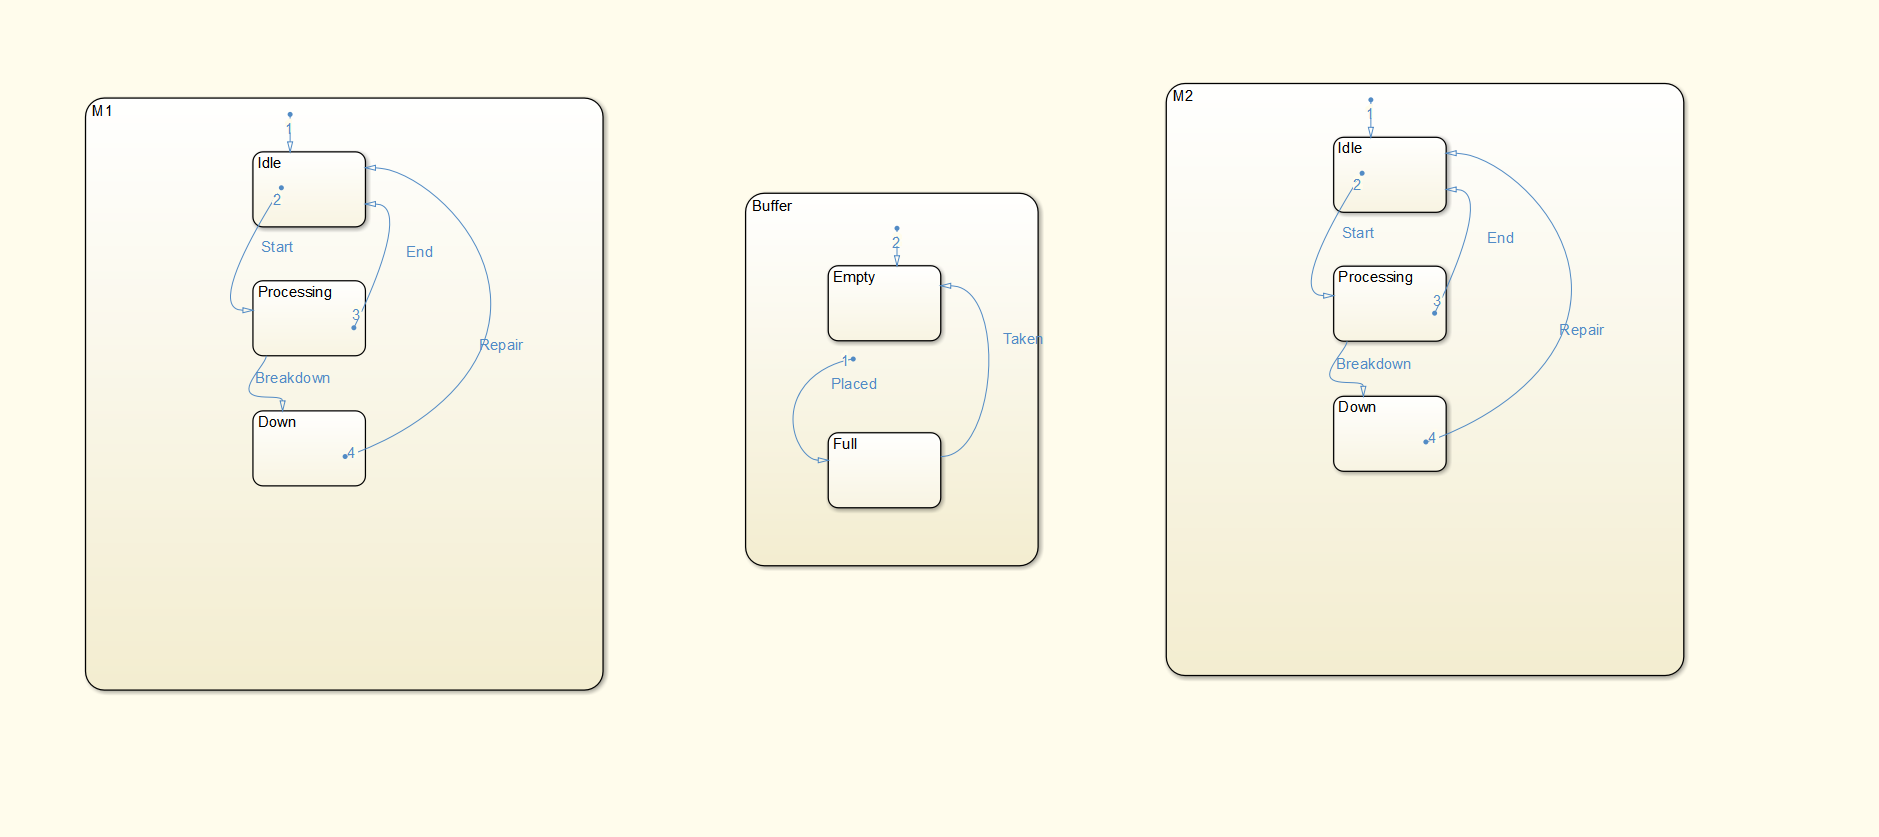
\includegraphics[width=1\linewidth]{../Matlab/HW2_sources_Windows64bit/images/task41_Chart.png}
        	\caption{Statechart of the three parallel systems.}
        	\label{fig:task41_Chart}
    \end{figure}	
}

\q % 2
{
	Construct and draw the complete DES that models $M_1$, $M_2$ and the $Buffer$ that models all behaviours of the system.
}
{

	In Figure~\ref{fig:task42_Chart} the full statechart can be seen. As all behaviours were not defined assumptions were made that only one state may change at a time, and therefore $PROCESSING$ triggers $FULL$ without changing its state.
	
	\begin{figure}[H]
    		\centering
        	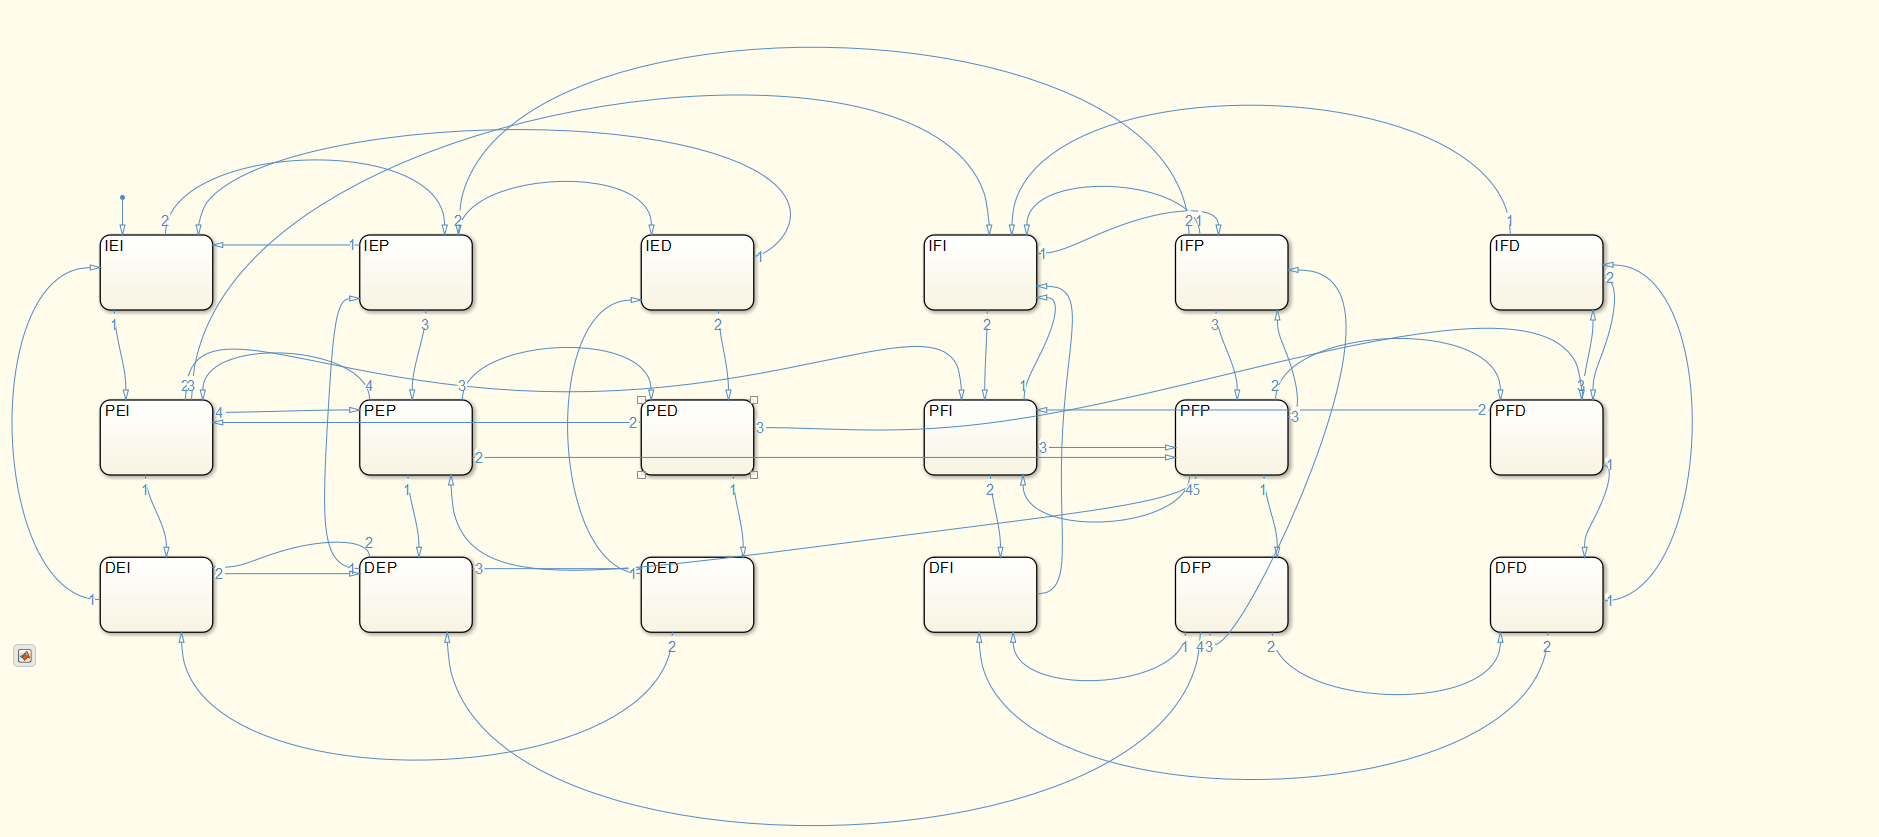
\includegraphics[width=1\linewidth]{../Matlab/HW2_sources_Windows64bit/images/task42_Chart.png}
        	\caption{Full statechart of all possible events and transition.}
        	\label{fig:task42_Chart}
    \end{figure}	
}

\q % 3
{
	Construct and draw the DES that models $M_1$, $M_2$ and $B$ with additional rules.
}
{

	In Figure~\ref{fig:task43_Chart} the full statechart with the added rules can be seen. 
	
	\begin{figure}[H]
    		\centering
        	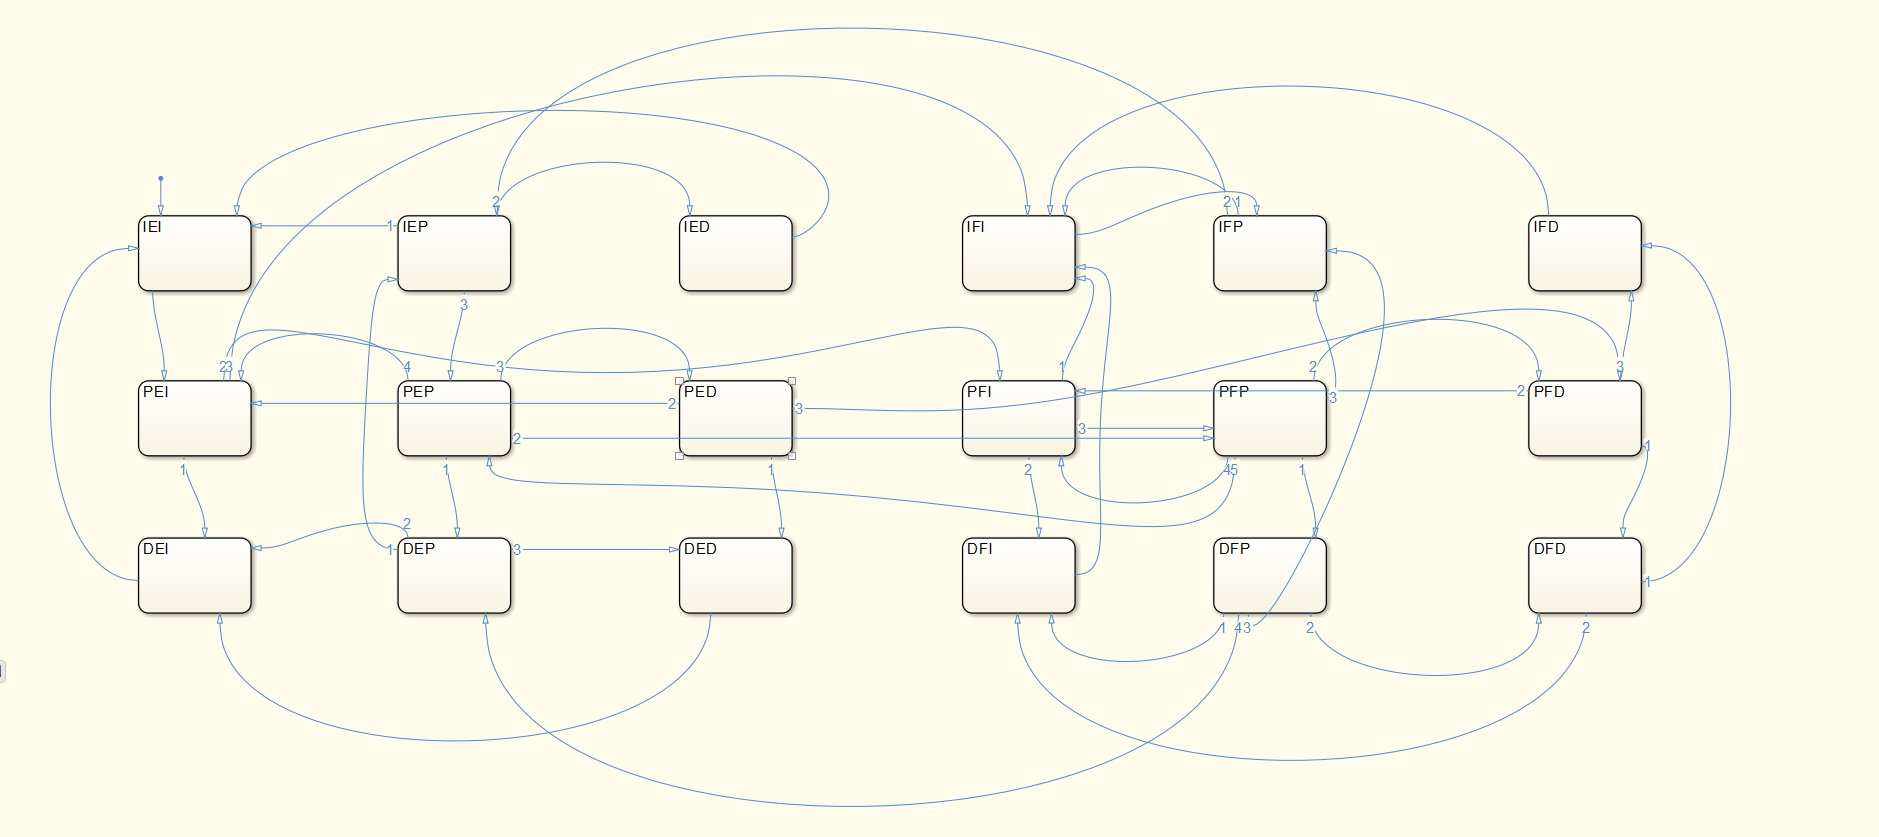
\includegraphics[width=1\linewidth]{../Matlab/HW2_sources_Windows64bit/images/task43_Chart.png}
        	\caption{Statechart of all possible events and transition with added rules.}
        	\label{fig:task43_Chart}
    \end{figure}	
}

\q % 4
{
	Adding the ability to enable or disable the events $START$ and $REPAIR$ describe this.
}
{

	Add two additional parallel pair of states with the states $START$ $ENABLED$ and $START$ $DISABLED$ for the first and $REPAIR$ $ENABLED$ and $REPAIR$ $DISABLED$ for the second. 
	
	Add guards on all transitions initiated by the events $START$ and $REPAIR$ which requires the associated parallel statemachine to be in its enabled state.
}

\end{document}
